\chapter{Eserciziario Risolto e Commentato Tipo-Esame}
\label{chap:eserciziario}

In questo capitolo presentiamo una selezione di esercizi d'esame accuratamente risolti e commentati, rappresentativi di tutte le tipologie di problemi assegnati nelle prove scritte del Prof. Cutolo. Per ciascun esercizio viene evidenziata la metodologia risolutiva generale e i passaggi formali attesi in sede di correzione.

% ------------------------------------------------------------------------------
\section{Studio di Relazioni di Equivalenza e Quozienti}

\begin{esercizio}{Relazione d'Equivalenza su $\Z \times \Z$}{es_equiv}
Sull'insieme $A = \Z \times \Z$ si consideri la relazione binaria $\mathcal{R}$ definita ponendo, per ogni $(a, b), (c, d) \in A$:
\[
    (a, b) \mathcal{R} (c, d) \quad \Shiff \quad a + 2d = c + 2b
\]
\begin{enumerate}
    \item Dimostrare che $\mathcal{R}$ è una relazione di equivalenza su $A$.
    \item Determinare esplicitamente la classe di equivalenza $[(0, 0)]_\mathcal{R}$ e la classe $[(1, 2)]_\mathcal{R}$.
    \item Descrivere geometricamente o algebricamente l'insieme quoziente $A/\mathcal{R}$.
\end{enumerate}
\end{esercizio}

\begin{proof}[Risoluzione Commentata]
\textbf{Punto 1: Verifica delle proprietà di equivalenza.}
Riscriviamo la condizione spostando le variabili con lo stesso indice:
\[
    a + 2d = c + 2b \quad \Shiff \quad a - 2b = c - 2d
\]
Definiamo l'applicazione ausiliaria $f: \Z \times \Z \to \Z$ ponendo $f(a, b) = a - 2b$.
Allora la relazione $\mathcal{R}$ coincide esattamente con il \textbf{nucleo di equivalenza} di $f$:
\[
    (a, b) \mathcal{R} (c, d) \quad \Shiff \quad f(a, b) = f(c, d)
\]
Poiché il nucleo di equivalenza di qualunque applicazione è una relazione di equivalenza (Definizione~\ref{def:nucleo_eq}), $\mathcal{R}$ è automaticamente riflessiva, simmetrica e transitiva!
\begin{itemize}
    \item \emph{Riflessività:} $\forall (a, b)$, $f(a, b) = f(a, b) \implies a - 2b = a - 2b \implies (a, b) \mathcal{R} (a, b)$.
    \item \emph{Simmetria:} se $f(a, b) = f(c, d)$, allora $f(c, d) = f(a, b)$, quindi $(c, d) \mathcal{R} (a, b)$.
    \item \emph{Transitività:} se $f(a, b) = f(c, d)$ e $f(c, d) = f(e, g)$, per transitività dell'uguaglianza in $\Z$ si ha $f(a, b) = f(e, g)$, da cui $(a, b) \mathcal{R} (e, g)$.
\end{itemize}

\textbf{Punto 2: Determinazione delle classi di equivalenza.}
Per definizione, la classe di $(x_0, y_0)$ è la fibra $\antivecf(\{f(x_0, y_0)\})$:
\begin{itemize}
    \item Per $(0, 0)$: $f(0, 0) = 0 - 0 = 0$. Dunque:
    \[
        [(0, 0)]_\mathcal{R} = \{(a, b) \in \Z \times \Z \mid a - 2b = 0\} = \{(2b, b) \mid b \in \Z\}
    \]
    È l'insieme di tutti i punti a coordinate intere giacenti sulla retta $a = 2b$.
    \item Per $(1, 2)$: $f(1, 2) = 1 - 2(2) = -3$. Dunque:
    \[
        [(1, 2)]_\mathcal{R} = \{(a, b) \in \Z \times \Z \mid a - 2b = -3\} = \{(2b - 3, b) \mid b \in \Z\}
    \]
\end{itemize}

\textbf{Punto 3: Struttura dell'insieme quoziente $A/\mathcal{R}$.}
Per il Teorema di Omomorfismo per insiemi (Teorema~\ref{teo:teo_omom_insiemi}), l'applicazione indotta:
\[
    \tilde{f}: (\Z \times \Z)/\mathcal{R} \longrightarrow \im(f), \qquad [(a, b)]_\mathcal{R} \longmapsto a - 2b
\]
è una \textbf{biiezione}.
Poiché per ogni $k \in \Z$ si ha $f(k, 0) = k - 0 = k$, l'applicazione $f$ è suriettiva su $\Z$, quindi $\im(f) = \Z$.
Ne deduciamo che l'insieme quoziente $(\Z \times \Z)/\mathcal{R}$ è in biiezione con $\Z$ (ha la cardinalità del numerabile $\aleph_0$), e ogni classe corrisponde a una retta discreta di pendenza $1/2$ nel reticolo $\Z^2$.
\end{proof}

% ------------------------------------------------------------------------------
\section{Studio di un Poset e Diagramma di Hasse}

\begin{esercizio}{Poset dei Divisori e Verifica di Reticolo}{es_poset}
Sia $S = \{2, 3, 4, 6, 8, 12, 24\}$ ordinato mediante la relazione di divisibilità $\mid$ ($a \le b \iff a \mid b$).
\begin{enumerate}
    \item Verificare che $(S, \mid)$ è un poset e tracciarne il diagramma di Hasse.
    \item Determinare gli elementi minimali, massimali, l'eventuale minimo e massimo di $S$.
    \item Stabilire se $(S, \mid)$ è un reticolo.
    \item Calcolare $\inf(4, 6)$ e $\sup(4, 6)$ in $S$.
\end{enumerate}
\end{esercizio}

\begin{proof}[Risoluzione Commentata]
\textbf{Punto 1: Diagramma di Hasse.}
La relazione di divisibilità su interi positivi è un ordine parziale (riflessiva, antisimmetrica, transitiva).
Troviamo le relazioni di copertura $x \prec y$ ($x \mid y$ senza divisori intermedi in $S$):
\begin{itemize}
    \item Da $2$: $2 \prec 4$ (non ci sono intermedi), $2 \prec 6$. (Non copre $8$ perché $2 \mid 4 \mid 8$).
    \item Da $3$: $3 \prec 6$.
    \item Da $4$: $4 \prec 8$, $4 \prec 12$.
    \item Da $6$: $6 \prec 12$.
    \item Da $8$: $8 \prec 24$.
    \item Da $12$: $12 \prec 24$.
\end{itemize}

Il diagramma di Hasse è illustrato di seguito:

\begin{center}
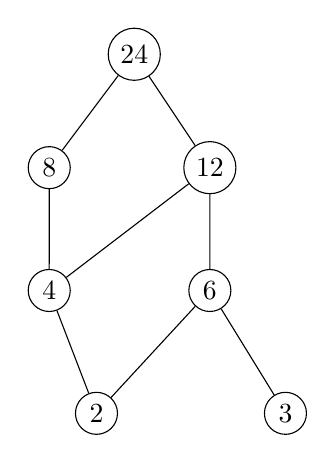
\begin{tikzpicture}[scale=1.2, every node/.style={circle, draw, fill=white, inner sep=2.5pt}]
    \node (2) at (-1, 0) {$2$};
    \node (3) at (1, 0) {$3$};
    \node (4) at (-1.5, 1.3) {$4$};
    \node (6) at (0.2, 1.3) {$6$};
    \node (8) at (-1.5, 2.6) {$8$};
    \node (12) at (0.2, 2.6) {$12$};
    \node (24) at (-0.6, 3.8) {$24$};
    
    \draw (2) -- (4);
    \draw (2) -- (6);
    \draw (3) -- (6);
    \draw (4) -- (8);
    \draw (4) -- (12);
    \draw (6) -- (12);
    \draw (8) -- (24);
    \draw (12) -- (24);
\end{tikzpicture}
\end{center}

\textbf{Punto 2: Elementi Speciali.}
\begin{itemize}
    \item \textbf{Minimali:} gli elementi che non hanno nulla al di sotto: $\{2, 3\}$.
    \item \textbf{Minimo:} non esiste alcun elemento che divida tutti gli elementi di $S$ contemporaneamente ($2 \nmid 3$ e $3 \nmid 2$). Dunque \textbf{non esiste minimo}.
    \item \textbf{Massimali:} l'unico elemento che non ha nulla al di sopra è $\{24\}$.
    \item \textbf{Massimo:} poiché $24$ è multiplo di tutti gli elementi di $S$ ($2, 3, 4, 6, 8, 12$ dividono tutti $24$), \textbf{$24$ è il massimo assoluto}: $\max(S) = 24$.
\end{itemize}

\textbf{Punti 3 e 4: Verifica di Reticolo.}
Per essere un reticolo, ogni coppia di elementi deve ammettere $\inf$ e $\sup$ \textbf{in $S$}.
Consideriamo la coppia $\{2, 3\}$:
I minoranti di $\{2, 3\}$ in $S$ sono: $\minor(\{2, 3\}) = \{x \in S \mid x \mid 2 \wedge x \mid 3\} = \vuoto$ (poiché l'unico divisore comune sarebbe $1$, ma $1 \notin S$).
Non essendovi minoranti in $S$, l'insieme $\minor(\{2, 3\})$ non può avere massimo, dunque \textbf{non esiste $\inf(2, 3)$ in $S$}.
Ne segue immediatamente che \textbf{$(S, \mid)$ non è un reticolo}!

Calcoliamo ora $\inf(4, 6)$ e $\sup(4, 6)$:
\begin{itemize}
    \item Minoranti di $\{4, 6\}$ in $S$: $\minor(\{4, 6\}) = \{x \in S \mid x \mid 4 \wedge x \mid 6\} = \{2\}$.
    Il massimo di tale insieme è $2$, quindi:
    \[
        \inf(4, 6) = 2
    \]
    \item Maggioranti di $\{4, 6\}$ in $S$: $\maggior(\{4, 6\}) = \{x \in S \mid 4 \mid x \wedge 6 \mid x\} = \{12, 24\}$.
    Il minimo di questo insieme è $12$, dunque:
    \[
        \sup(4, 6) = 12
    \]
\end{itemize}
\end{proof}

% ------------------------------------------------------------------------------
\section{Equazione Congruenziale Lineare con Algoritmo di Bézout}

\begin{esercizio}{Risoluzione Completa di Congruenza Lineare}{es_congr}
Si consideri l'equazione congruenziale lineare:
\[
    72x \equiv 42 \pmod{102}
\]
\begin{enumerate}
    \item Stabilire se l'equazione ammette soluzioni e quante soluzioni distinte modulo $102$ esistono.
    \item Determinare tutte le soluzioni intere in $\Z$ e tutte le soluzioni modulo $102$.
\end{enumerate}
\end{esercizio}

\begin{proof}[Risoluzione Commentata]
\textbf{Passo 1: Calcolo di $d = \mcd(72, 102)$ con l'algoritmo euclideo.}
Eseguiamo le divisioni successive:
\begin{align*}
    102 &= 72 \cdot 1 + 30 \\
    72 &= 30 \cdot 2 + 12 \\
    30 &= 12 \cdot 2 + 6 \\
    12 &= 6 \cdot 2 + 0 \quad (\text{resto nullo})
\end{align*}
L'ultimo resto non nullo è $d = 6$. Dunque $\mcd(72, 102) = 6$.
Poiché $d = 6$ divide il termine noto $42$ ($42 = 6 \cdot 7$), per il Criterio di Solvibilità (Teorema~\ref{teo:solv_congr}) l'equazione \textbf{è risolubile} e ammette esattamente \textbf{$6$ soluzioni distinte modulo $102$}.

\textbf{Passo 2: Semplificazione dell'equazione.}
Dividiamo tutti i termini per $d = 6$:
\[
    \frac{72}{6} x \equiv \frac{42}{6} \pmod{\frac{102}{6}} \quad \Implica \quad 12x \equiv 7 \pmod{17}
\]
I coefficienti $12$ e $17$ sono coprimi: $\mcd(12, 17) = 1$.

\textbf{Passo 3: Calcolo dell'inverso di $12$ modulo $17$ con l'identità di Bézout.}
Eseguiamo le divisioni tra $17$ e $12$:
\begin{align*}
    17 &= 12 \cdot 1 + 5 \\
    12 &= 5 \cdot 2 + 2 \\
    5 &= 2 \cdot 2 + 1
\end{align*}
Risaliamo a ritroso per esprimere $1$ come combinazione lineare di $17$ e $12$:
\begin{align*}
    1 &= 5 - 2 \cdot 2 \\
    &= 5 - 2 \cdot (12 - 5 \cdot 2) = 5 \cdot 5 - 2 \cdot 12 \\
    &= 5 \cdot (17 - 12 \cdot 1) - 2 \cdot 12 = 5 \cdot 17 - 7 \cdot 12
\end{align*}
Abbiamo ottenuto l'identità di Bézout:
\[
    17 \cdot 5 + 12 \cdot (-7) = 1
\]
Passando modulo $17$:
\[
    12 \cdot (-7) \equiv 1 \pmod{17}
\]
Poiché $-7 \equiv 10 \pmod{17}$, l'inverso di $12$ modulo $17$ è $[10]_{17}$.

\textbf{Passo 4: Soluzione particolare.}
Moltiplichiamo entrambi i membri di $12x \equiv 7 \pmod{17}$ per l'inverso $10$:
\[
    x_0 \equiv 10 \cdot 7 = 70 \equiv 2 \pmod{17} \quad (\text{poiché } 70 = 17 \cdot 4 + 2)
\]
Dunque una soluzione particolare è $x_0 = 2$.

\textbf{Passo 5: Tutte le $6$ soluzioni modulo $102$.}
Le $d = 6$ soluzioni distinte modulo $102$ si ottengono aggiungendo multipli di $m' = 17$:
\[
    x_k = x_0 + k \cdot 17 \qquad \text{per } k \in \{0, 1, 2, 3, 4, 5\}
\]
Calcoliamo esplicitamente:
\begin{align*}
    x_0 &= 2 \\
    x_1 &= 2 + 17 = 19 \\
    x_2 &= 19 + 17 = 36 \\
    x_3 &= 36 + 17 = 53 \\
    x_4 &= 53 + 17 = 70 \\
    x_5 &= 70 + 17 = 87
\end{align*}
Le classi di equivalenza delle soluzioni in $\Z_{102}$ sono $\{[2], [19], [36], [53], [70], [87]\}$.
L'insieme di tutte le soluzioni intere in $\Z$ è:
\[
    S = \{2 + 17k \mid k \in \Z\}
\]
\end{proof}

% ------------------------------------------------------------------------------
\section{Calcolo di Grandi Potenze Modulari}

\begin{esercizio}{Calcolo Potenze con Eulero-Fermat}{es_potenza}
Determinare il resto della divisione di $13^{2026}$ per $35$.
\end{esercizio}

\begin{proof}[Risoluzione Commentata]
Vogliamo calcolare $13^{2026} \pmod{35}$.
\begin{enumerate}
    \item \textbf{Verifica della coprimarità:} La fattorizzazione in primi di $35$ è $35 = 5 \cdot 7$.
    Poiché $13$ non è divisibile né per $5$ né per $7$, si ha $\mcd(13, 35) = 1$.
    Possiamo quindi applicare il \textbf{Teorema di Eulero-Fermat}.
    \item \textbf{Calcolo di $\varphi(35)$:} Per la proprietà moltiplicativa:
    \[
        \varphi(35) = \varphi(5) \cdot \varphi(7) = (5 - 1) \cdot (7 - 1) = 4 \cdot 6 = 24
    \]
    Per il teorema: $13^{24} \equiv 1 \pmod{35}$.
    \item \textbf{Divisione dell'esponente per $\varphi(35) = 24$:}
    \[
        2026 = 24 \cdot 84 + 10 \qquad (\text{resto } 10)
    \]
    \item \textbf{Riduzione dell'esponente:}
    \[
        13^{2026} = (13^{24})^{84} \cdot 13^{10} \equiv 1^{84} \cdot 13^{10} \equiv 13^{10} \pmod{35}
    \]
    \item \textbf{Calcolo rapido di $13^{10} \pmod{35}$:}
    \begin{align*}
        13^2 &= 169 = 35 \cdot 4 + 29 \equiv -6 \pmod{35} \\
        13^4 &= (13^2)^2 \equiv (-6)^2 = 36 \equiv 1 \pmod{35} \\
        13^8 &= (13^4)^2 \equiv 1^2 = 1 \pmod{35} \\
        13^{10} &= 13^8 \cdot 13^2 \equiv 1 \cdot (-6) = -6 \equiv 29 \pmod{35}
    \end{align*}
\end{enumerate}
Il resto cercato è quindi $29$.
\end{proof}

% ------------------------------------------------------------------------------
\section{Fattorizzazione di Polinomi in $\Z_p[x]$ e Campi Quoziente}

\begin{esercizio}{Irriducibilità e Quoziente in $\Z_3[x]$}{es_polinomio}
In $\Z_3[x]$, si consideri il polinomio $f(x) = x^3 + 2x + 1$.
\begin{enumerate}
    \item Determinare se $f(x)$ è irriducibile in $\Z_3[x]$.
    \item Stabilire se l'anello quoziente $K = \Z_3[x]/(f(x))$ è un campo e calcolarne la cardinalità $|K|$.
    \item Nel quoziente $K$, determinare l'inverso moltiplicativo dell'elemento $[x]$.
\end{enumerate}
\end{esercizio}

\begin{proof}[Risoluzione Commentata]
\textbf{Punto 1: Studio dell'irriducibilità.}
Il polinomio $f(x)$ ha grado $3$. Per la Proposizione~\ref{prop:criterio_grado_2_3}, un polinomio di terzo grado a coefficienti in un campo è irriducibile se e solo se non possiede radici nel campo.
Valutiamo $f(x)$ in tutti gli elementi di $\Z_3 = \{0, 1, 2\}$:
\begin{align*}
    f(0) &= 0^3 + 2(0) + 1 = 1 \not\equiv 0 \pmod 3 \\
    f(1) &= 1^3 + 2(1) + 1 = 1 + 2 + 1 = 4 \equiv 1 \not\equiv 0 \pmod 3 \\
    f(2) &= 2^3 + 2(2) + 1 = 8 + 4 + 1 = 13 \equiv 1 \not\equiv 0 \pmod 3
\end{align*}
Poiché $f(c) \neq 0$ per ogni $c \in \Z_3$, $f(x)$ \textbf{non ha radici in $\Z_3$}.
Essendo di terzo grado, ne deduciamo che \textbf{$f(x)$ è irriducibile in $\Z_3[x]$}.

\textbf{Punto 2: Natura e cardinalità del quoziente.}
Per il Teorema~\ref{teo:campo_quoziente}, poiché $f(x)$ è irriducibile su un campo, l'anello quoziente:
\[
    K = \Z_3[x]/(f(x))
\]
è un \textbf{campo} (noto come campo finito o estensione di Galois $\F_{3^3} = \F_{27}$).
I suoi elementi sono rappresentati univocamente dai polinomi di grado strettamente minore di $\degpoly(f) = 3$:
\[
    K = \{a_0 + a_1 x + a_2 x^2 + (f(x)) \mid a_0, a_1, a_2 \in \Z_3\}
\]
Poiché ci sono 3 scelte indipendenti per ciascuno dei 3 coefficienti ($a_0, a_1, a_2$), la cardinalità è:
\[
    |K| = 3^3 = 27 \text{ elementi}
\]

\textbf{Punto 3: Calcolo dell'inverso di $[x]$ in $K$.}
Nel quoziente vale la relazione $[f(x)] = [0]$, cioè:
\[
    [x^3 + 2x + 1] = [0] \quad \Implica \quad [x^3 + 2x] = [-1] = [2]
\]
Raccogliendo $[x]$ a fattor comune a sinistra:
\[
    [x] \cdot [x^2 + 2] = [2]
\]
Moltiplichiamo entrambi i membri per l'inverso di $2$ in $\Z_3$ (che è $2$, poiché $2 \cdot 2 = 4 \equiv 1 \pmod 3$):
\[
    [x] \cdot [2(x^2 + 2)] = [2 \cdot 2] = [1]
\]
Poiché $2(x^2 + 2) = 2x^2 + 4 \equiv 2x^2 + 1 \pmod 3$, otteniamo:
\[
    [x]^{-1} = [2x^2 + 1]
\]
Verifica immediata: $x(2x^2 + 1) = 2x^3 + x = 2(-2x - 1) + x = -4x - 2 + x = -3x - 2 \equiv -2 \equiv 1 \pmod 3$.
\end{proof}
